% main.tex — حواف العدّ والحساب — Prime
% نسخة Overleaf من prime.tex — نفس المحتوى تمامًا، والاسم main.tex لأن Overleaf يترجم main.tex افتراضيًا.
% يُترجم بـ XeLaTeX (وليس pdfLaTeX)، بخط Amiri المتوفر في Overleaf TeX Live.
% الصور — بأسماء القايمة في Overleaf (سلسلة B، حسب وصف الصور في HTML):
% primeB1.png = D1 | primeB2.png = الكثافة | primeB3.png = تكرار الحواف
% لا توجد صورة بطاقة هوية ولا رسم أول 2000 حافة في القايمة، فحُذفت هاتان الصورتان من الملف.
\documentclass[12pt,a4paper]{article}
% ترتيب الحزم مهم: كل الحزم قبل polyglossia، لأنها تحمّل bidi.
\usepackage{fontspec}
\usepackage{amsmath,amssymb}
\usepackage{graphicx}
\usepackage{booktabs}
\usepackage{array}
\usepackage[margin=2.2cm]{geometry}
\usepackage{xcolor}
\usepackage{fancyhdr}
\usepackage{polyglossia}
\setmainlanguage[numerals=maghrib]{arabic}
\setotherlanguage{english}
\setmainfont{Amiri}

% ترقيع لتوافق bidi في TeX Live الحديث: \@tabular يستدعي هذا الأمر، وهو غير معرّف في بعض الإصدارات.
\AtBeginDocument{\providecommand{\UseMathForPositioningText}{}}

% الفوتر: يظهر في كل الصفحات، بما فيها الأولى.
\pagestyle{fancy}
\fancyhf{}
\fancyfoot[C]{عبدالله الجبري — حواف العدّ والحساب — Prime — \thepage}
\renewcommand{\headrulewidth}{0pt}
\renewcommand{\footrulewidth}{0pt}

\title{حواف العدّ والحساب — Prime}
\author{عبدالله الجبري}
\date{نوفمبر 2026م}

\begin{document}
\maketitle
\thispagestyle{fancy}
\begin{center}
\textbf{نعدّ الأوليات، نحسب حوافها، ونختبر ما إذا كانت تحمل بنية أو ذاكرة.}
\end{center}



\section{الهوية الرسمية}

\begin{table}[h]
\centering
\begin{tabular}{ll}
\toprule
العنصر & المعتمد \\
\midrule
الاسم & حواف العدّ والحساب \\
الرمز & \textenglish{Prime} \\
التعريف الرياضي & $g_n = p_{n+1} - p_n$ \\
المنهج & استخراج الأوليات، ثم حساب الحواف، ثم تحليلها \\
السؤال البحثي & هل للفجوات ذاكرة؟ \\
\bottomrule
\end{tabular}
\end{table}

\section{التعريف والاشتقاق}

\subsection{الحافة}

\textbf{الحافة = الفرق بين أوليين متتاليين:}

\[
g_n = p_{n+1} - p_n
\]

\subsection{كيف تُحسب الحافة؟ — ثلاث خطوات لا غير}

\begin{enumerate}
\item \textbf{الغربال:} غربال إراتوستينس لاستخراج الأوليات حتى $N$، مع استبعاد العدد 1 صراحةً.
\item \textbf{الفرق:} كل حافة هي الفرق بين أوليين متتاليين.
\item \textbf{الحافة الأولى:} $3 - 2 = 1$ — الحالة الابتدائية الوحيدة الفردية. جميع الحواف التالية زوجية، لأن كل أولي بعد 2 فردي، والفرق بين فرديين زوجي.
\end{enumerate}

\subsection{مثال مصغر}

\begin{table}[h]
\centering
\begin{tabular}{ccc}
\toprule
الأولي الحالي & الأولي التالي & الحافة \\
\midrule
2 & 3 & 1 \\
3 & 5 & 2 \\
5 & 7 & 2 \\
7 & 11 & 4 \\
11 & 13 & 2 \\
\bottomrule
\end{tabular}
\end{table}

\subsection{دوال العدّ والانحراف}

\begin{itemize}
\item $\pi(x)$ = عدد الأوليات $\leq x$.
\item $\mathrm{Li}(x) = \mathrm{Ei}(\ln x) - \mathrm{Ei}(\ln 2) = \int_2^x \frac{dt}{\ln t}$.
\item المرجع الثاني: $x / \ln x$.
\item $D_1(x) = \pi(x) - \mathrm{Li}(x)$.
\item $D_2(x) = \pi(x) - x/\ln x$.
\item $R(x) = |D_1(x)| / \pi(x)$.
\item $\rho_k = (\pi(b_k) - \pi(a_k)) / 10^8$ — كثافة النافذة $k$.
\item $\bar{g}_k = 1 / \rho_k$ — متوسط الحافة في النافذة $k$.
\item $\Delta D_1$ = تغيّر $D_1$ عن نقطة القياس السابقة.
\end{itemize}

\subsection{قاعدة العدّ في D}

الحافة تُقبل داخل D فقط عندما يكون طرفها الأعلى أكبر من 100M.

\subsection{فئات M1}

\begin{itemize}
\item صغيرة: $g \leq 6$.
\item متوسطة: $8 \leq g \leq 14$.
\item كبيرة: $g \geq 16$.
\end{itemize}

«متوسطة 8–14» دقيقة تمامًا: الحافة الفردية الوحيدة هي 1، وهي صغيرة، فلا توجد حافة 7 أو 15 أصلًا.

\section{الحسابات المعتمدة — D: من 100M إلى 1B}

\subsection{الجدول التراكمي — كل 100 مليون}

\begin{table}[h]
\centering
\small
\begin{tabular}{rrrrrrr}
\toprule
$x$ & $\pi(x)$ & $\mathrm{Li}(x)$ & $D_1$ & $\Delta D_1$ & $D_2$ & $R(x)$ \\
\midrule
$100{,}000{,}000$ & $5{,}761{,}455$ & $5{,}762{,}208.3$ & $-753.3$ & $-753.3$ & $332{,}774.0$ & $0.000131$ \\
$200{,}000{,}000$ & $11{,}078{,}937$ & $11{,}079{,}973.8$ & $-1{,}036.8$ & $-283.5$ & $615{,}308.2$ & $0.000094$ \\
$300{,}000{,}000$ & $16{,}252{,}325$ & $16{,}253{,}408.1$ & $-1{,}083.1$ & $-46.3$ & $882{,}915.9$ & $0.000067$ \\
$400{,}000{,}000$ & $21{,}336{,}326$ & $21{,}337{,}377.0$ & $-1{,}051.0$ & $+32.1$ & $1{,}141{,}420.0$ & $0.000049$ \\
$500{,}000{,}000$ & $26{,}355{,}867$ & $26{,}356{,}831.1$ & $-964.1$ & $+86.9$ & $1{,}393{,}458.7$ & $0.000037$ \\
$600{,}000{,}000$ & $31{,}324{,}703$ & $31{,}326{,}044.207$ & $-1{,}341.207$ & $-377.103$ & $1{,}640{,}014.082$ & $0.000042816$ \\
$700{,}000{,}000$ & $36{,}252{,}931$ & $36{,}254{,}240.999$ & $-1{,}309.999$ & $+31.208$ & $1{,}882{,}917.694$ & $0.000036135$ \\
$800{,}000{,}000$ & $41{,}146{,}179$ & $41{,}147{,}861.2$ & $-1{,}682.2$ & $-372.2$ & $2{,}122{,}021.5$ & $0.000041$ \\
$900{,}000{,}000$ & $46{,}009{,}215$ & $46{,}011{,}647.6$ & $-2{,}432.6$ & $-750.4$ & $2{,}357{,}836.0$ & $0.000053$ \\
$1{,}000{,}000{,}000$ & $50{,}847{,}534$ & $50{,}849{,}233.912$ & $-1{,}699.912$ & $+732.688$ & $2{,}592{,}591.566$ & $0.000033432$ \\
\bottomrule
\end{tabular}
\end{table}

\begin{figure}[h]
\centering
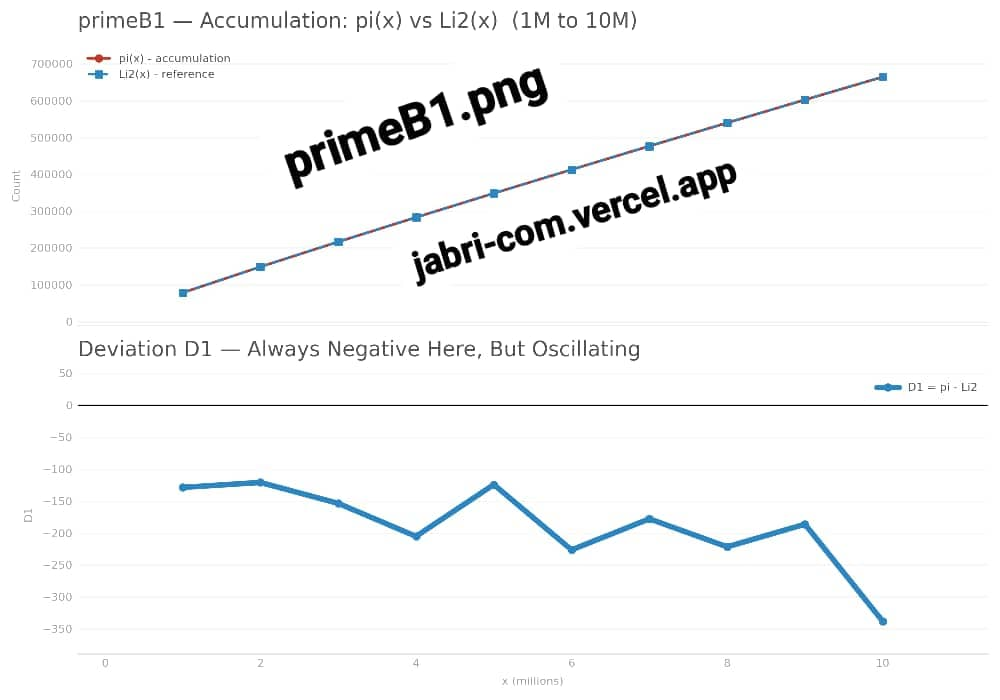
\includegraphics[width=0.95\textwidth]{primeB1.png}
\caption{$D_1$ عبر نقاط D العشر}
\end{figure}

\textbf{قراءة:} $D_1$ بقي سالبًا في كل نقاط D (π أقل من Li). $\Delta D_1$ تذبذب بين $-750.4$ و $+732.7$، ولم يغيّر إشارة $D_1$. $R$ تذبذب بين $0.000033$ و $0.000094$، وأغلق عند 1B على $0.000033$ — الأدنى في السلسلة كلها.

\subsection{الكثافة المحلية في نوافذ D التسع}

\begin{table}[h]
\centering
\begin{tabular}{rrrr}
\toprule
النافذة & أوليات النافذة & $\rho_k$ & $\bar{g}_k = 1/\rho_k$ \\
\midrule
100M – 200M & $5{,}317{,}482$ & $0.053175$ & $18.806$ \\
200M – 300M & $5{,}173{,}388$ & $0.051734$ & $19.330$ \\
300M – 400M & $5{,}084{,}001$ & $0.050840$ & $19.670$ \\
400M – 500M & $5{,}019{,}541$ & $0.050195$ & $19.922$ \\
500M – 600M & $4{,}968{,}836$ & $0.049688$ & $20.125$ \\
600M – 700M & $4{,}928{,}228$ & $0.049282$ & $20.291$ \\
700M – 800M & $4{,}893{,}248$ & $0.048932$ & $20.436$ \\
800M – 900M & $4{,}863{,}036$ & $0.048630$ & $20.563$ \\
900M – 1B & $4{,}838{,}319$ & $0.048383$ & $20.668$ \\
\bottomrule
\end{tabular}
\end{table}

\begin{figure}[h]
\centering
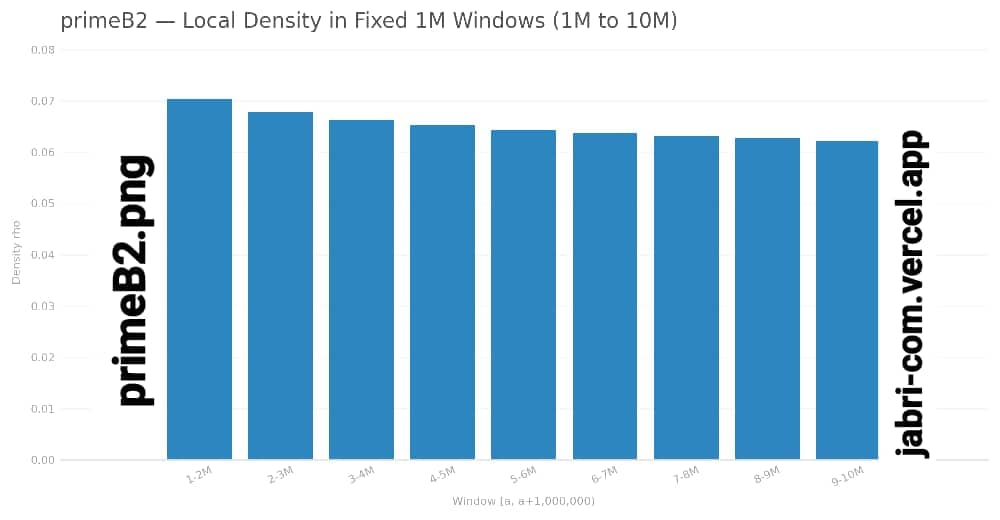
\includegraphics[width=0.95\textwidth]{primeB2.png}
\caption{الكثافة في نوافذ D}
\end{figure}

\textbf{قراءة:} الكثافة تنخفض في كل نافذة من D: من $0.053175$ عند 100–200M إلى $0.048383$ عند 900M–1B. الانخفاض مستمر لكنه يتباطأ: الفرق بين أول نافذتين $\approx 0.00144$، وبين آخر نافذتين $\approx 0.00025$.

\subsection{الفجوات داخل D فقط}

\textbf{إجمالي الفجوات المحسوبة في D = 45,086,079.}

\begin{table}[h]
\centering
\begin{tabular}{rrr}
\toprule
المرتبة & الفجوة & التكرار في D \\
\midrule
1 & 6 & $5{,}321{,}039$ \\
2 & 12 & $3{,}930{,}575$ \\
3 & 10 & $3{,}054{,}751$ \\
4 & 4 & $2{,}984{,}422$ \\
5 & 2 & $2{,}984{,}194$ \\
6 & 18 & $2{,}966{,}294$ \\
7 & 8 & $2{,}360{,}929$ \\
8 & 14 & $2{,}171{,}364$ \\
9 & 24 & $2{,}109{,}926$ \\
10 & 30 & $1{,}955{,}144$ \\
11 & 16 & $1{,}630{,}293$ \\
12 & 20 & $1{,}621{,}121$ \\
13 & 22 & $1{,}393{,}734$ \\
14 & 28 & $1{,}089{,}676$ \\
15 & 36 & $1{,}057{,}496$ \\
\bottomrule
\end{tabular}
\end{table}

\begin{figure}[h]
\centering
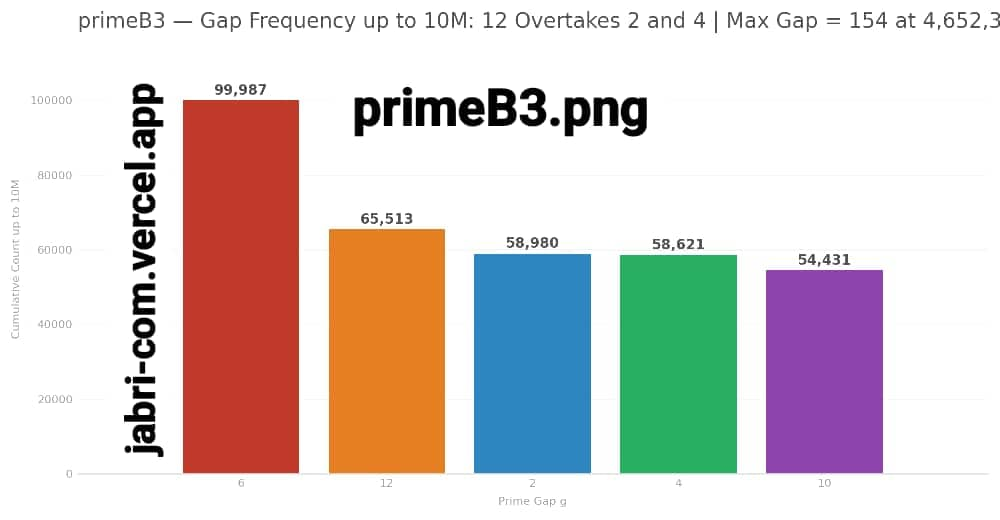
\includegraphics[width=0.95\textwidth]{primeB3.png}
\caption{تكرار الحواف الخمس عشرة الأولى في D}
\end{figure}

\textbf{قراءة بلا تفسير قسري:}
\begin{itemize}
\item الترتيب الجديد في D: 6، 12، 10، 4، 2، 18، 8، 14، 24، 30 \dots
\item 12 بقيت في المرتبة الثانية.
\item 10 تقدّمت من المرتبة الخامسة (في الترتيب التراكمي حتى 100M: 6، 12، 2، 4، 10، 18) إلى الثالثة في D.
\item المسافة بين تكرار 2 و 4 تقلّصت جدًا في D: $2{,}984{,}194$ مقابل $2{,}984{,}422$ — فرق 228 فقط.
\item لم تظهر فجوة جديدة في قائمة الأكثر تكرارًا؛ القائمة العليا نفسها، لكن ترتيبها تغيّر.
\item لا نفترض ثبات الترتيب بعد D.
\end{itemize}

\textbf{أكبر فجوة في D: 282}، بين 436,273,009 و 436,273,291، داخل النافذة الخامسة (400M–500M).

\subsection{سجل التحقق المستقل — Prime D: VERIFIED}

\begin{itemize}
\item تحقق مستقل بغربال مجزّأ مستقل، يستبعد 1 صراحةً من مجموعة الأوليات.
\item طابقت جميع نقاط العدّ التراكمي العشر.
\item طابقت جميع أعداد النوافذ التسع.
\item إجمالي عدد الأوليات عبر النوافذ التسع: 45,086,079.
\item التصحيحان +1 المُبلّغ عنهما سابقًا عند 600M و 700M \textbf{مرفوضان}.
\item طابق ترتيب تكرار الفجوات الخمس عشرة الأولى.
\item تأكّدت أكبر فجوة 282 بين 436,273,009 و 436,273,291.
\item الأعداد التراكمية الأصلية وحدود النوافذ والبروتوكول الحسابي بقيت كما هي.
\item سبب الخلاف السابق: خطأ في غربال التحقق المستقل الذي احتسب 1 ضمن الأوليات — لا عيب في الحساب الأصلي.
\end{itemize}

\section{M1 — موثّق}

\textbf{السؤال:} هل فئة حجم الفجوة الحالية تحمل معلومة عن فئة الفجوة التالية؟

\textbf{النموذج:} Markov-1 على فئات الحجم. الحالة = فئة حجم الفجوة، ومصفوفة الانتقال التجريبية:

\[
P_{ab} = \Pr(S_{i+1} = b \mid S_i = a)
\]

\textbf{النتيجة:} $r = -0.03006$ — «الكبير يتبعه الصغير».

ارتباط سلبي ضعيف جدًا في الاختبار الحالي، وليس قانونًا تنبؤيًا. النتيجة لا تدعم حتى الآن وجود ارتباط قوي يمكن الاعتماد عليه للتنبؤ بالفجوة التالية. نحتفظ بها كما هي، دون تعديل الفئات أو إعادة تعريف الاختبار لتناسب نتيجة مرغوبة.

\section{M1-E — مجمّدة، بانتظار \textenglish{gaps.csv}}

\textbf{السؤال:} هل الفجوة الدقيقة تحمل معلومات انتقالية إضافية لم تستطع الفئات الثلاث التقاطها؟

\subsection{ملف الإدخال}

\textenglish{gaps.csv} عمود واحد فقط، حافة في كل سطر.

\begin{itemize}
\item رأس اختياري: \textenglish{gap} أو \textenglish{g} أو \textenglish{gaps}.
\item أي عمود إضافي يُرفض.
\item أي سطر غير رقمي يوقف التشغيل بموضعه — لا حذف صامت أبدًا.
\item أي فجوة غير صالحة توقف التشغيل بموضعها.
\end{itemize}

\subsection{البروتوكول المجمّد}

\begin{itemize}
\item التقسيم على الانتقالات نفسها: أول 50\% من الانتقالات تدريب، وآخر 50\% اختبار، والانتقال على الحد الفاصل لا يسقط.
\item الفجوات حتى 30: قيمة دقيقة. فوق 30: نطاقات لوغاريتمية محددة مسبقًا: 30، 44، 62، 88، 124، 176، 248، 350، 500.
\item عتبة الدمج: 200 مشاهدة في التدريب، من بيانات التدريب فقط.
\item قاعدة الدمج: أي نطاق دون 200 يُدمج مع النطاق الأعلى التالي. الاستثناء: النطاق الأخير يبقى كما هو ولا يُدمج نزولًا.
\item Laplace smoothing: alpha = 1 على عدّادات الانتقال بعد الدمج.
\item Bootstrap: كتل متجاورة دائرية بطول ثابت، كتلة = 100 انتقال، B = 2000، فاصل 95\%. كل عينة Bootstrap طولها عدد انتقالات الاختبار.
\item الحكم: تحسن Log-Loss وتفسير Pearson مقياسان منفصلان.
\item عدم التحسن لا يثبت غياب المعلومات.
\item فاصل Bootstrap يقيس عدم يقين إعادة أخذ عينات الاختبار مع تثبيت النماذج المدرّبة، لا عدم يقين إعادة التدريب.
\item محاكاة Pearson بحرق بداية 2000 خطوة حتى استقرار السلسلة.
\item البذرة: SEED = 20261120.
\item الحدود المقبولة وحدها: 6، 14 — الحدود 10/30 كانت افتراضًا من الكاتب، وهي الآن مرفوضة.
\end{itemize}

\subsection{التشغيل}

\begin{verbatim}
python3 m1e_tomorrow_final.py gaps.csv --classes 6,14
\end{verbatim}

مرة واحدة على \textenglish{gaps.csv}، دون تعديل بعد ظهور النتيجة. الوضع التجريبي (\textenglish{--demo}، حتى 300,000) تجربة فقط، وليس الاختبار الفعلي.

\section{المحاكاة — أداة استكشاف فقط}

\textenglish{prime-id.html} — بطاقة + إدخال $N$ + جدول عند قوى 10 + رسم الفجوات.

\textbf{الفصل مهم:} النتائج المرجعية حتى مليار محفوظة كما اعتمدت، أما المحاكاة فهي أداة استكشاف، ولا يجوز أن تعيد إنتاج الأرقام المرجعية بطريقة تقريبية ثم تخلطها بها.

\textbf{حدود المحاكاة الموثّقة:}
\begin{itemize}
\item \textenglish{Li2(x)} يستخدم تكامل Simpson بعدد تقسيم ثابت (8000). عند إدخال $10^6$ فما فوق لا يُعامل ناتجه على أنه دقيق — الخطأ في $D_1$ عند $10^6$ هو $-43.31$، وعند $10^7$ هو $-509.26$.
\item \textenglish{sieve(N)} يستهلك ذاكرة تنمو خطيًا مع $N$ (\textenglish{Uint8Array(N+1)}: عند $10^7$ $\approx$ 10 MB فوق مصفوفة الأوليات)، وهو سبب حقيقي لثقل المتصفح عند الرفع.
\item \textenglish{primes.filter(p<=x)} يعيد فحص قائمة الأوليات لكل صف في الجدول.
\item الرسم الحالي يرسم الفجوات وفق ترتيبها، لكنه لا يمثل تحليلًا دوريًا أو كشفًا لنمط؛ إنه رسم وصفي فقط.
\end{itemize}



\section{ما لم نثبته — خط أحمر}

\begin{itemize}
\item لا: قانون دوري لتذبذب الفجوات.
\item لا: تفسير رياضي لترتيب الفجوات.
\item لا: ضمان استمرار $D_1$ سالبًا بعد المليار.
\item لا: قانون تنبؤي من M1.
\item لا: نظرية جديدة للأعداد الأولية مستنتجة من هذه النتائج.
\end{itemize}

\section{حالة المشروع}

\begin{table}[h]
\centering
\begin{tabular}{ll}
\toprule
العنصر & الحالة \\
\midrule
Prime — المرحلة الحالية & النتائج محفوظة \\
المسح حتى مليار & مكتمل \\
M1 (فئات 6، 14) & موثّق \\
M1-E & مجمّدة، بانتظار \textenglish{gaps.csv} \\
التفسير النظري & غير محسوم \\
\bottomrule
\end{tabular}
\end{table}

\section{الملفات}

\begin{table}[h]
\centering
\begin{tabular}{ll}
\toprule
الملف & الدور \\
\midrule
\textenglish{prime-d.html} & سجل D المغلق والموثّق — الجداول والتحقق المستقل \\
\textenglish{m1e\_tomorrow\_final.py} & سكربت M1-E المجمّد — البروتوكول والاختبار \\
\textenglish{prime-id.html} & المحاكاة — بطاقة + استكشاف (ليست مصدر الأرقام المرجعية) \\
\textenglish{README.md} & الهوية والاشتقاقات والحسابات والصور \\
\textenglish{main.tex} & هذا الملف — نسخة Overleaf من \textenglish{prime.tex} \\
\bottomrule
\end{tabular}
\end{table}

\vspace{1em}
\begin{center}
\textbf{لا نطارد نتيجة، ولا نُجبر الأرقام على صناعة نظرية.}

لدينا رصد حتى مليار، وأربعون نقطة، واتجاهات قابلة للمقارنة، واختبارات محفوظة. هذه قاعدة جيدة للعمل القادم، حتى لو لم تعطنا القانون الذي نبحث عنه بعد.

\textbf{الحافة بسيطة. ما قد تحمله هو السؤال الحقيقي.} 
\end{center}

\end{document}
